% !TeX root = ../../Parte4.tex
\secmeme{node/logout}
\section[Sessioni]{Gestione delle sessioni}\transfade\centering
\begin{frame}{Sessione}
  La sessione permette di salvare (sul server) dei dati associati ad un client.\smallskip\\\pause
  Questi dati vengono persi quando il browser viene chiuso, a meno che non sia impostata una data di scadenza diversa sul server.\pause\bigskip\\
  \alert{Attenzione!} L'abbinamento client-sessione avviene salvando un cookie nel browser, pertanto se si usano le sessioni bisogna mostrare un avviso all'utente secondo le norme del GDPR.
\end{frame}
\begin{frame}[fragile]\transfade\centering
  \begin{enumerate}
    \item \mint{bash}{npm add express-session && npm install}
    \item {\small\texttt{server.js}:}
    \begin{minted}{js}
const express = require('express');
const session = require('express-session');

const app = express();
const port = 3000;

app.use(session({
    resave: false, // non salvare la sessione se non avvengono modifiche
    saveUninitialized: false, // non creare sessioni vuote
    secret: '$Ks!U97F%434DL&r^%B7o' // chiave con cui viene criptata la sessione
}));

app.get('/', (req, res) => {
    if(req.session.visualizzazioni) // se `visualizzaioni' è membro della sessione
        ++req.session.visualizzazioni;
    else
        req.session.visualizzazioni = 1;
    res.send(`Pagina visualizzata ${req.session.visualizzazioni} volte.`);
})

app.listen(port);
    \end{minted}
    \item \texttt{\small npm start}
  \end{enumerate}
\end{frame}

\begin{frame}
  \begin{figure}
    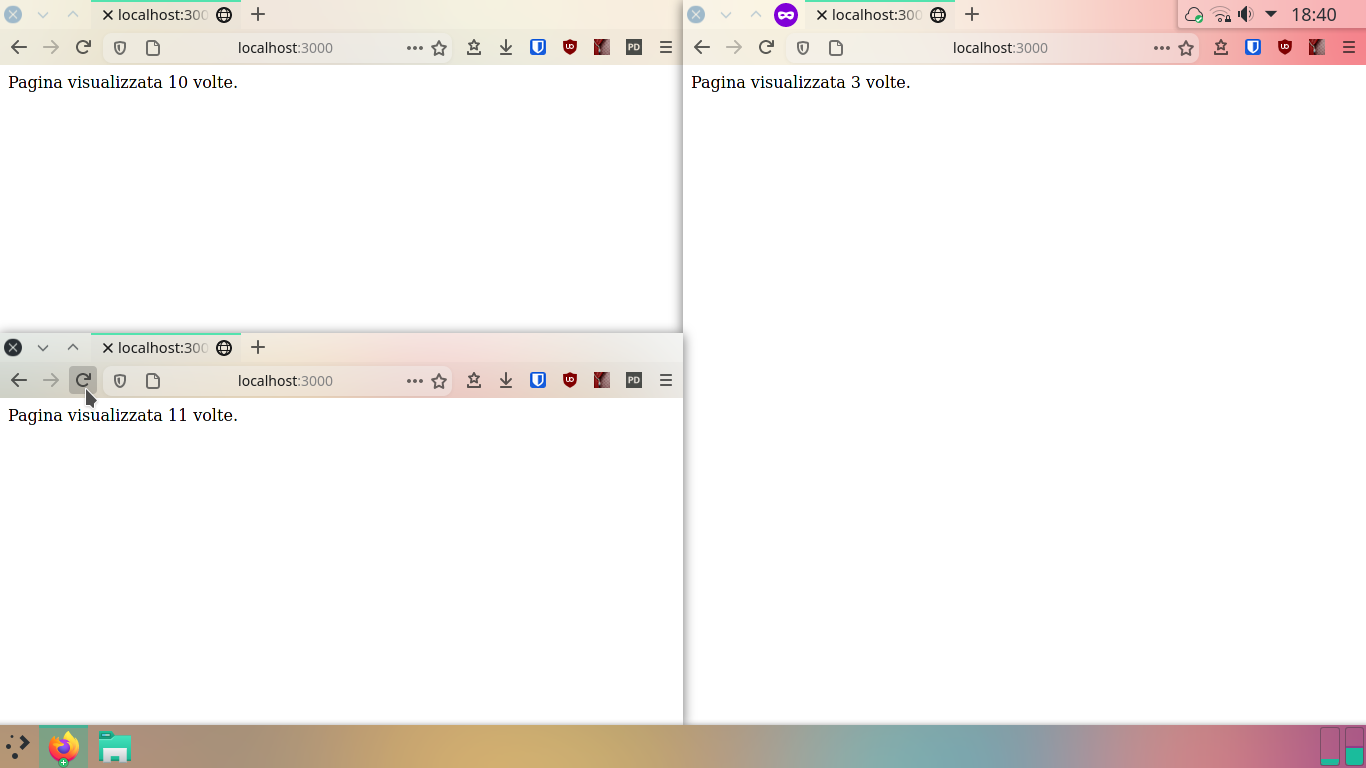
\includegraphics[height=.8\paperheight]{img/node/session}
    \caption{La sessione è unica del profilo di un browser: ad esempio usando la navigazione in incognito la sessione è diversa.}
  \end{figure}
\end{frame}